%%%%%%%%%%%%%%%%%%%%%%%%%%%%%%%%%%%%%%%%%%%%%%%%%%%%%%%%%%%%%%%%%%%%%%%%%%%%%%%%%%%%%%%%%%%%%%%%
%
% CS484 Written Question Template
%
% Acknowledgements:
% The original code is written by Prof. James Tompkin (james_tompkin@brown.edu).
% The second version is revised by Prof. Min H. Kim (minhkim@kaist.ac.kr).
%
% This is a LaTeX document. LaTeX is a markup language for producing 
% documents. Your task is to fill out this document, then to compile 
% it into a PDF document. 
%
% 
% TO COMPILE:
% > pdflatex thisfile.tex
%
% If you do not have LaTeX and need a LaTeX distribution:
% - Personal laptops (all common OS): www.latex-project.org/get/
% - We recommend latex compiler miktex (https://miktex.org/) for windows,
%   macTex (http://www.tug.org/mactex/) for macOS users.
%   And TeXstudio(http://www.texstudio.org/) for latex editor.
%   You should install both compiler and editor for editing latex.
%   The another option is Overleaf (https://www.overleaf.com/) which is 
%   an online latex editor.
%
% If you need help with LaTeX, please come to office hours. 
% Or, there is plenty of help online:
% https://en.wikibooks.org/wiki/LaTeX
%
% Good luck!
% Min and the CS484 staff
%
%%%%%%%%%%%%%%%%%%%%%%%%%%%%%%%%%%%%%%%%%%%%%%%%%%%%%%%%%%%%%%%%%%%%%%%%%%%%%%%%%%%%%%%%%%%%%%%%
%
% How to include two graphics on the same line:
% 
% \includegraphics[\width=0.49\linewidth]{yourgraphic1.png}
% \includegraphics[\width=0.49\linewidth]{yourgraphic2.png}
%
% How to include equations:
%
% \begin{equation}
% y = mx+c
% \end{equation}
% 
%%%%%%%%%%%%%%%%%%%%%%%%%%%%%%%%%%%%%%%%%%%%%%%%%%%%%%%%%%%%%%%%%%%%%%%%%%%%%%%%%%%%%%%%%%%%%%%%

\documentclass[11pt]{article}

\usepackage[english]{babel}
\usepackage[utf8]{inputenc}
\usepackage[colorlinks = true,
            linkcolor = blue,
            urlcolor  = blue]{hyperref}
\usepackage[a4paper,margin=1.5in]{geometry}
\usepackage{stackengine,graphicx}
\usepackage{fancyhdr}
\setlength{\headheight}{15pt}
\usepackage{microtype}
\usepackage{times}
\usepackage{booktabs}

% From https://ctan.org/pkg/matlab-prettifier
\usepackage[numbered,framed]{matlab-prettifier}

\frenchspacing
\setlength{\parindent}{0cm} % Default is 15pt.
\setlength{\parskip}{0.3cm plus1mm minus1mm}

\pagestyle{fancy}
\fancyhf{}
\lhead{Homework Writeup}
\rhead{CS484}
\rfoot{\thepage}

\date{}

\title{\vspace{-1cm}Homework 3 Writeup}


\begin{document}
\maketitle
\vspace{-3cm}
\thispagestyle{fancy}

\section*{Instructions}
\begin{itemize}
  \item Describe any interesting decisions you made to write your algorithm.
  \item Show and discuss the results of your algorithm.
  \item Feel free to include code snippets, images, and equations.
  \item Use as many pages as you need, but err on the short side If you feel you only need to write a short amount to meet the brief, th
  
  \item \textbf{Please make this document anonymous.}
\end{itemize}

\section*{In the beginning...}

In this project, I implement stereo-imaging by calculating disparity map from 2 bayer images. In my project, there are 2 interesting points. \\
\\
1) Using "imregcorr" for alignment of two rectified images,\\
2) Using guided filter for cost aggregation.\\


\section*{Interesting Implementation Detail}

For arranging the two rectified images, I use the Matlab function imregcorr(), which estimates geometric transformation that aligns two 2-D images using phase correlation. The affine2d tform calculated by imregcorr() is applied to one of rectified images by imwarp().

\begin{lstlisting}[style=Matlab-editor]
%calculate the affine2d for translate rectified1 
%to well aligned with rectified2.
tform = imregcorr(rectified1, rectified2, 'translation');

%pad 2 images for preserving the images after the
%translation.
delta = tform.T;
d_x = floor(abs(delta(3,1)));
d_y = floor(abs(delta(3,2)));
rectified1 = padarray(rectified1, [d_y,d_x]);
rectified2 = padarray(rectified2, [d_y,d_x]);


%apply the translation at rectified1.
Rout = affineOutputView(size(rectified1), tform, 'BoundsStyle', 'SameAsInput');
rectified1 = imwarp(rectified1, tform, 'OutputView', Rout);
\end{lstlisting}


For cost aggregation, the guided filter is used. Guided filter is one of the popular filter in stereo imaging, because it preserves the image's edge with fast computation\cite{6012131}. Here, I use self-guidance, where the image is filter while guided by itself.

\begin{lstlisting}[style=Matlab-editor]
for i=1:max_disparity
    cost_vol(:,:,i) = imguidedfilter(cost_vol(:,:,i)); 
end
\end{lstlisting}

\section*{A Result}

\begin{enumerate}
    \item Result 1 (Figure~\ref{fig:result1})was a total failure, because the two rectified images are not aligned well. Here the box filter is used for cost aggregation.
    \item Result 2 (Figure~\ref{fig:result2}) was successful, because the two rectified images are aligned well. Here the box filter is used for cost aggregation.
    \item Result 3 (Figure~\ref{fig:result3}) is a little clearer than result2, because it uses the guided filter, not the box filter.
\end{enumerate}

\begin{figure}[h]
    \centering
    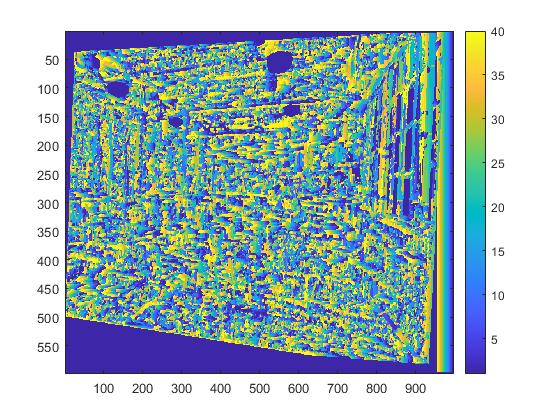
\includegraphics[width=13cm]{writeup/box filter.jpg}
    \caption{Result 1}
    \label{fig:result1}
\end{figure}

\begin{figure}[h]
    \centering
    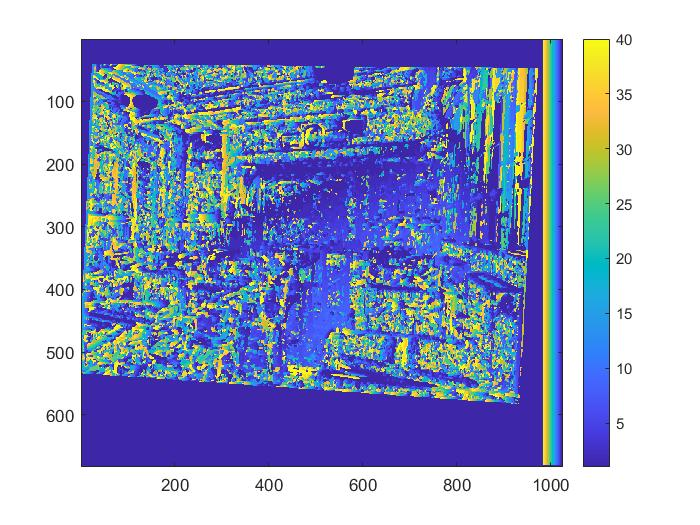
\includegraphics[width=13cm]{writeup/box filter success.jpg}
    \caption{Result 2}
    \label{fig:result2}
\end{figure}

\begin{figure}[h]
    \centering
    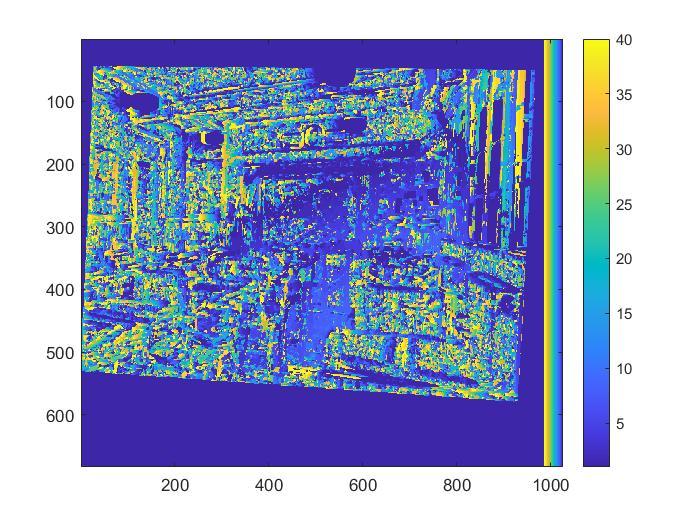
\includegraphics[width=13cm]{writeup/guided filter with no guidance.jpg}
    \caption{Result 3}
    \label{fig:result3}
\end{figure}

Times taken for cost aggregation with 1) box filter (BF) and 2) guided filter (GF) are compared in Table~\ref{tab:table1}. Although GF is fast edge preserving filter, BF is faster than GF because of its simple implementation.


\begin{table}[h]
    \centering
    \begin{tabular}{lrr}
        \toprule
        Filter & Trial1 & Trial2 \\
        \midrule
        BF & 0.4s & 0.3s\\
        GF & 2.6s & 2.7s\\
        \bottomrule
    \end{tabular}
    \caption{speed difference of the two filter.}
    \label{tab:table1}
\end{table}

\bibliographystyle{IEEEtran}
\bibliography{IEEEabrv, my.bib}

\end{document}